\label{chap5}

In this chapter the proposed model-based controller is tuned and verified in simulation and for experiments. First the models response to a free oscillation is shown. This can already be used to detect strengths and weaknesses of the dynamic model. Then the performance of the model-based controller will be evaluated for a reference set-point in simulation. Then the step to the experimental set-up is made. The experimental set-up will be discussed, including it's data acquisition using the sensory devices. Subsequently, the input mapping is reviewed. Next, the response for a set-point regulation with the model-based controller and filters will be presented. Lastly, the results of a reference tracking problem conducted on the experimental setup are shown. 



\section{Dynamic model in free-oscillation}

still work out, script finished

\section{Set-point regulation in simulation}

The controller of 


\section{Experimental set-up and data acquisition}

The experimental set-up consisting of the planar soft robot, air pumps, air tanks, and pressure sensors are connected as followed. Each air pump is attached to an air distribution manifold via a hose. This distribution manifold has three air outlets. To these outlets a pressure sensor, air tank and actuator bellow is attached, respectively. To this end, air hoses with a inner diameter of 3 millimeter are used. To the tip of the actuator a yellow LED is mounted that is used for optical tracking. This LED is glued to a connector that has been additively manufactured. The LED has an offset of 35 millimeter with respect the tip of the actuator. This connector part also houses the IMU. This IMU is used to measure rotation of the actuator's tip in degrees. Furthermore, a vision system is focused on the actuator. This vision system is programmed such it can recognise and track the LED marker. The actual end-effector position can then be calculated using trigonometry using rotation and position data, see Appendix \ref{app:chap5} for this derivation. 

The sensors described above, e.g. the IMU, two pressure sensors and optical tracking system are connected to an Arduino micro. This Arduino is connected to a Raspberry PI 3B+. The Arduino code is programmed such that it updates all sensors. This includes the optical tracking system, two pressure sensors and the IMU. The maximum attained sample frequency of the Arduino is 40 Hz. On the Raspberry the model-based and pressure controller are programmed. To the Raspberry a ADC converter shield is mounted which can regulate the input to the air pumps. The Raspberry PI is able to receive sensor data and perform all necessary calculations at a frequency of 25 Hz. This is the bandwidth frequency of the control system. This sample frequency of 25 Hz might seem low compared to traditional robots. However, considering the low system dynamics in the order of 1 Hz \cite{tawk2018bioinspired},\cite{HighBandwidthControl} this sample frequency suffices.  

\section{Digital filter design}

Since sensory devices are prone to measurement noise and disturbances digital filters are implemented. For the IMU two different filters are applied. For the pressure and visions systems a single filter suffices. 

For the IMU two filters are used to decrease noise and disturbances. First, the angle is filtered using a complementary filter, then a moving average filter is applied. The IMU consists of multiple sensors. One of these sensors is the accelerometer, which is able to measure acceleration based on force. An on-board gyroscope allows the measurement of rotational velocity. The output of both sensors can be used to calculate rotation on all 3 axis. Both sensors have their deficits. The accelerometer utilizes force to determine acceleration. This also includes actuation forces, hence undesired high frequent pump dynamics may influence the accelerometer readings. The gyroscope, on the other side, is prone to drift which becomes a problem over time. A complementary filter can be used to enhance angle calculations as this filter fuses gyroscopic data with acceleration data. To remove high frequent noise the acceleration data is low-pass filtered, whereas gyroscope data is high-pass filtered. Therefore, the complementary filter can be described as, 

\begin{equation}
    \theta_{} = \delta \theta_{acc} + (1-\delta) \int_0^t \omega_{gyr} \hspace{2pt} ds    \hspace{25pt} \text{with}  \hspace{10pt} \theta_{acc} = \atantwo(a_y,a_x)
\end{equation}

where $\theta_{acc}$ is calculated from the measured accelerations $a_y$ and $a_x$ in the IMU's y-direction and x-direction, respectively. The rotational velocity $\omega_{gyr}$ is measured by the IMU's gyroscope. Parameter $\delta \in 0 < \delta < 1$ determines the relative importance between acceleration and gyroscope data. Since the output of the IMU was not deemed satisfactory with the complementary filter, a moving average filter is implemented. With the complementary filter, high amplitude oscillatory angle changes where observed, whilst the tip of the soft robot was nearly constant. This moving average filter reduces the amplitude of the oscillations as previous angle data is used in the calculation. The moving average filter is given as,

\begin{equation}
    \Bar{\theta}_k = \frac{1}{N_{IMU}}\sum_{i = 0} ^ {N_{IMU}-1} \theta_{k-i}
\end{equation}

where $\Bar{\theta}_k$ is the averaged output, $N$ the amount of past samples to average and $\theta_k-i$ the past past sample. It must noted that both filters cause delays in the system. Therefore the tuning should be done carefully, as stability is not guaranteed.

The vision system which tracks the LED marker gives out its position data in pixels. These pixels are integer numbers, causing steps in the position measurement. To remove these steps and represent the average position during a sampling instant the data is low-pass filtered. This casts the integers pixels to doubles, thereby describing the average position during a sample instant better. The description of the low-pass filter is identical to (\ref{eq4:lowpass}) and given as,

\begin{equation}
\bar{r}_{pixy,k} = \zeta_{pixy} r_{pixy,k} + (1-\zeta_{pixy})\bar{k}_{pixy,k-1}
\label{eq5:lowpass}
\end{equation}

where $\Bar{r}_{pixy,k}$ is the low-pass filtered position vector of the LED marker given in pixels. The sampled position vector is $r_{pixy,k}$ and $\bar{k}_{pixy,k-1}$ the previous filtered position. Parameter $\zeta$ determines the cut-off frequency of the low-pass filter. High values for $\zeta$ prioritize recent samples, whereas low values stress past LED positions. The pressure data is also low-pass filtered, following an identical procedure as the position data. 


\section{Revision of input mapping}

The input mapping as derived in Chapter \ref{chap3} given by (\ref{eq3:H}) was found inaccurate during the experiments. Recall that this mapping maps moment and force to individual bellow pressure. Incorrect mapping results in erroneous pressure set points. The revised input mapping was found as follows. First, the pressure controller gains are set as $K_{pp} =\text{diag}([1,1])$ and the integrator gain $K_{ip} = \text{diag}([0,0])$. In this way, the system pressure will never converge to the pressure set point. Then a setpoint is chosen for which the soft robot needs to elongate and curve. Eventually, the soft robot will move to its desired position set point, as the integrator action in the model-based controller will increase $\nu_{set}$. Once the reference position is reached, the input signal $\nu_{set}$ remains constant. Furthermore, the pressure in both bellows can be read. Based on the pressures, and value of $\nu_{set}$ the entries of the input mapping can be redetermined. The revised input mapping was found to be equal to,

\begin{equation}
    H = \begin{bmatrix} 	0.0206 &  -0.0206 \\ 
	0.1808 & 0.1808 \end{bmatrix},
    \label{eq4:revisedH}
\end{equation}

where it can be seen that the moment to pressure mapping was off by a factor 10. The force mapping was of equal order. 

\section{Tuning procedure}


Table \ref{tab5:tuningcosiderations} shows the experimentally implemented tuning parameters together with its tuning consideration. The used parameters are found by iterative tuning and observing the system's response. This is done according to some procedure, which is detailed.

Initially, the proportional gains $K_{pp}$ of the pressure controller are set as $\text{diag}([1,1])$. The integrator gains $K_{ip}$ are left as $\text{diag([0,0])}$. Subsequently, the low-pass filter gains on the sensors $\zeta_p$, $\zeta_{pixy}$ are set relatively high ($>0.9$), to minimize delays. Likewise, the sample amount of the moving average filter $N_{IMU}$ can be chosen low ($<5$). The complementary filter $\delta_{IMU}$ is taken initially as 0.02 \cite{compfilter}. These values allow to pass trough almost all recent data without much delay. Then the curvature set-point as $r_{set} = [0.014,0.082]^\top$ is selected. The proportional gains of the Jacobian controller $K_p$ are increased, such that the system does not saturate in the first few seconds of its response. Recall that the first entry $K_{p,1}$ affects the moment, and $K_{p,2}$ induces a force. Increasing the value of $K_{p,1}$ will result in a swing-like motion in the first seconds, caused by the initially large error in x-direction. To minimize this behaviour gain $K_{p,1}$ should be chosen smaller than $K_{p,2}$. At this point, the integrator gain of the pressure controller $K_{ip}$ can be increased, to allow tracking the pressure set point. Furthermore, the integrator gains $K_i$ can be tuned, these should be chosen relatively high to decrease position error relatively fast. The integrator gains are chosen too high when overshoot is observed. Since the system can not be actively deflated, and deflation rates are low, the integrator is not able to compensate well for overshoot. Next the low-pass filter of the Jacobian controller $\zeta$ can be tuned. This parameter should be decreased to obtain a smooth input signal. At this point $\zeta_{pixy}$ can be tuned as well, to obtain a smoother position signal. Once the control input is smooth, the pressure response is considered. This response can be smoothed by decreasing the low-pass gain $\zeta_p$. Lastly, the sample amount $N_{IMU}$ of the moving average filter is tuned. This value should be tuned such that the angle settling time coincides with the error settling time. Once this procedure is completed, the system can be further fine tuned to increase performance. Table \ref{tab:tuningcosiderations} shows some guidelines and considerations whilst tuning the controller.


\begin{table}[H]
    \centering
     \caption{Tuning considerations experimental tuning}
    \begin{tabular}{p{2.5cm} p{9cm} p{3cm}} \hline
      \textbf{Parameter}   & \textbf{Tuning  consideration} & \textbf{Value [Unit]} \\ \hline
      $K_p$   &   $K_{p,1}$ affects curvature, whereas $K_{p,2}$ influences elongation. To decrease a swing like motion $K_{p,1} < K_{p,2}$. Motor saturation should be considered whilst tuning.   &  diag([$1750,3750$])     $[N] \And [N/m]$        \\ \hline
      $K_i$   &   $K_{i,1}$ acts on the moment, to compensate for lower gain, this parameter can be increased. When the gains $K_p$ are set, $K_i$ can be increased up until error overshoot occurs.   &  diag([$6500,6250$])  $[N] \And [N/m]$     \\ \hline
      $K_{pp}$   &  Is a scalar matrix due to assumed equal pump characters. It is not recommended to chose $K_p >1$ as this results in poor performance. Smaller values will result in a smoother volt input at the cost of performance.  &  diag([$1 ,1$]) $[V/kPa]$      \\ \hline
      $K_{ip}$   &  The integrator gains should be chosen such that system pressure tracks the reference pressure signal. If chosen too high, the system will still saturate the first few seconds.      &  diag([$0.75,0.75$]) $[V/kPa]$   \\ \hline
      $\zeta$    &   This parameter allows to create smooth reference control input. A weigh-off is made between smoothness and delays. &  $0.08$ $[-]$ \\ \hline
      $\zeta_p$    &   This parameter has a major influence the control input. A smooth pressure reading will result in a smoother control input $V$. Low values will result in stability problems.   & $0.25$ $[-]$  \\ \hline
      $\zeta_{pixy}$    &  Since the vision system uses discretized pixel coordinates, a filter can be used to estimate position during a sample instant. Delays should be considered and minimized     & $0.25$  $[-]$ \\ \hline
      $N_{IMU}$    &  This value should be picked such that large oscillation in the angle readings are minimized, whilst reducing the delay as much as possible. & $35$ $[-]$  \\ \hline
      $\delta_{IMU}$    &  High values stress importance of accelerometer readings, low values emphasize gyroscopic data. Since the actuator forces affect accelerometer readings it is recommended not to pick $\delta_{IMU}$ too high.  & $0.08$ $[-]$ \\ \hline
    \end{tabular}

    \label{tab5:tuningcosiderations}
\end{table}



\section{Set-point regulation in experiments}


The performance of the designed controller is assessed by analyzing the system's response whilst moving to a reference position. Two set-points are considered for which the actuator needs to extend and curve. The first set-point is $r_{set} = [-0.014,0.082] m$, the second set-point is mirrored and given by $r_{set} = [0.014,0.082] m$. These set-points enable analyzing the movement in both Cartesian directions, due to symmetry it is assumed that the step-responses are alike.


Figure \ref{fig5:stepleft} shows the error signal as a function of time in x and y direction, respectively. The lower plot 







\newpage
\begin{figure}[H]
    \centering
    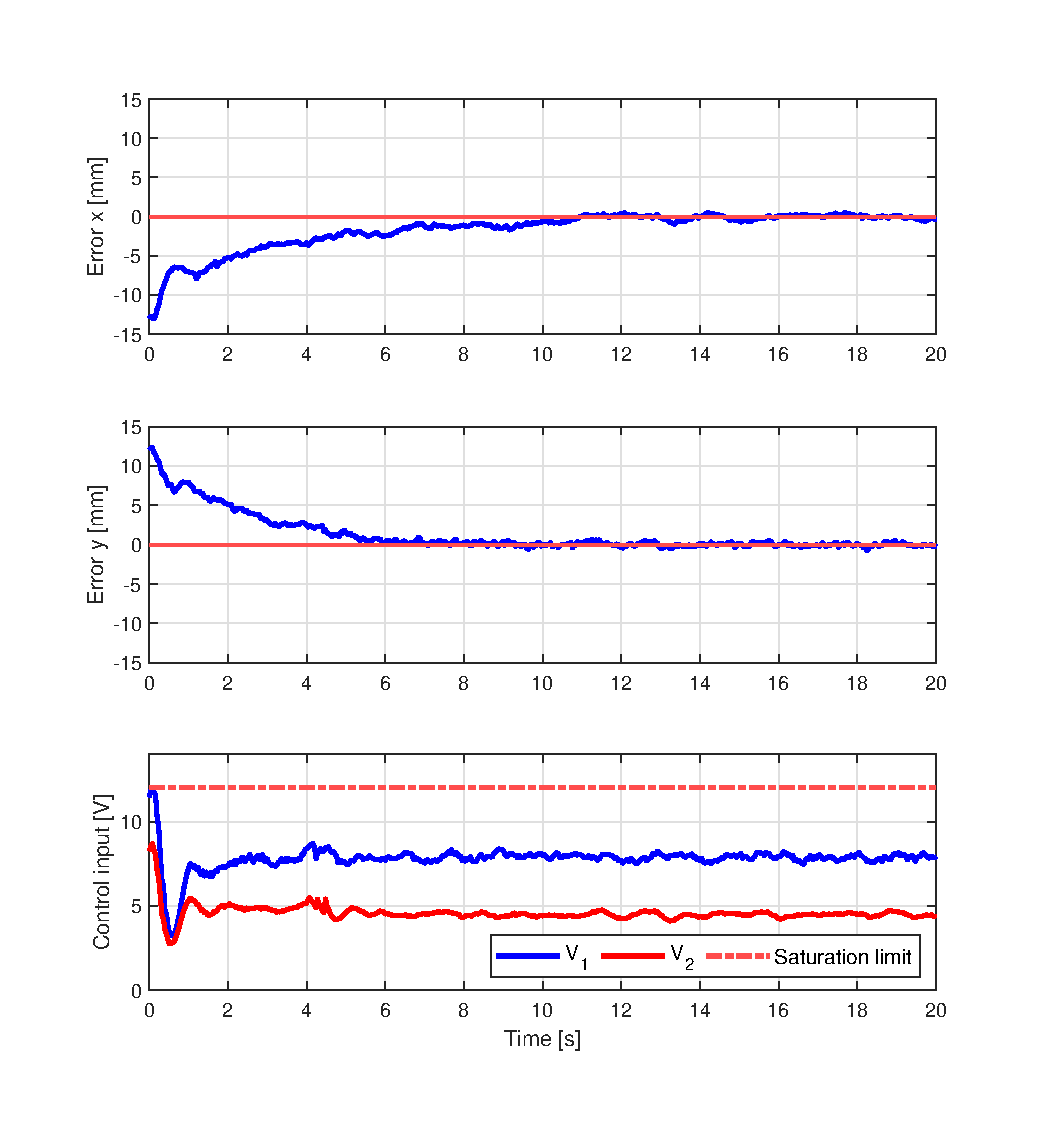
\includegraphics[width = \textwidth]{Figures/Chapter5/errorsignalleftwide.eps}
    \caption{\textbf{Top:} Error response of the x-coordinate. \textbf{Centre:} Error response of the y-coordinate. \textbf{Bottom:} Control input signal to the air-pumps.}
    \label{fig5:stepleft}
\end{figure}

\begin{figure}[H] 
    \begin{minipage}[b]{0.49\linewidth}
     \centering
    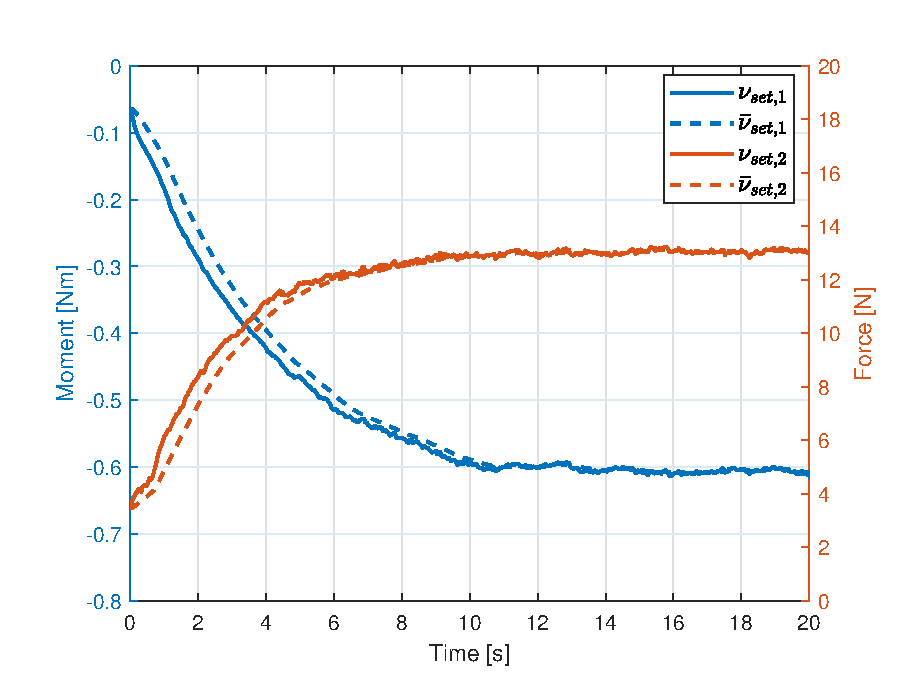
\includegraphics[width=\linewidth]{Figures/Chapter5/nuleft.eps} 
    \caption{Input moment and force as determined by Jacobian controller. Solid line is unfiltered input, dotted line low-pass filtered. } 
    \label{fig3:dim} 
       \end{minipage} 
    \begin{minipage}[b]{0.49\linewidth}
     \centering
    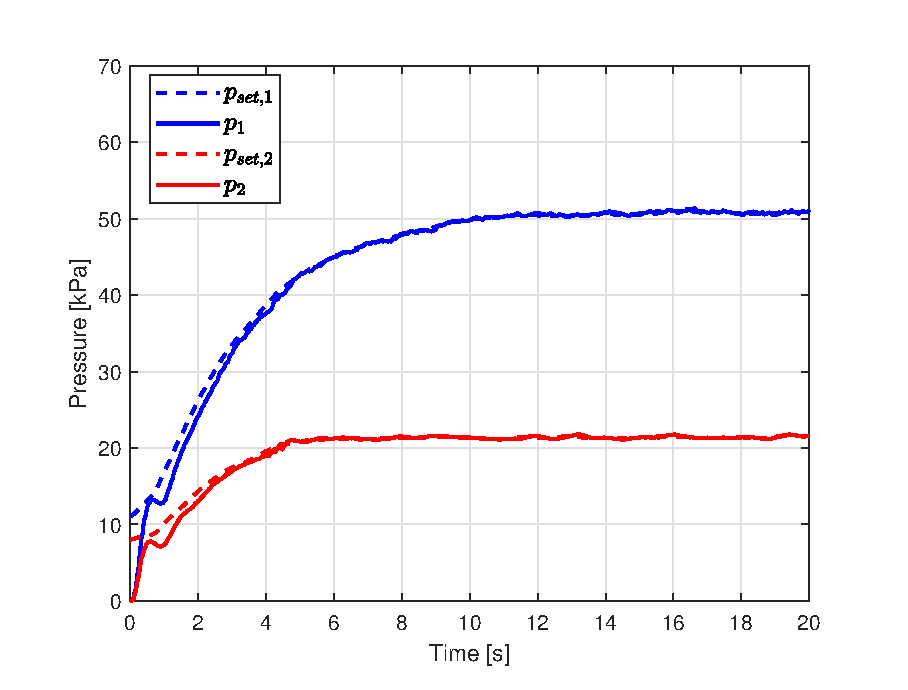
\includegraphics[width=\linewidth]{Figures/Chapter5/pressureleft.eps} 
    \caption{Pressure response, dotted lines indicate reference pressure, solid lines are measured pressures.} 
    \label{fig3:FemModel} 
    \end{minipage} 
\end{figure}




\newpage
\begin{figure}[H]
    \centering
    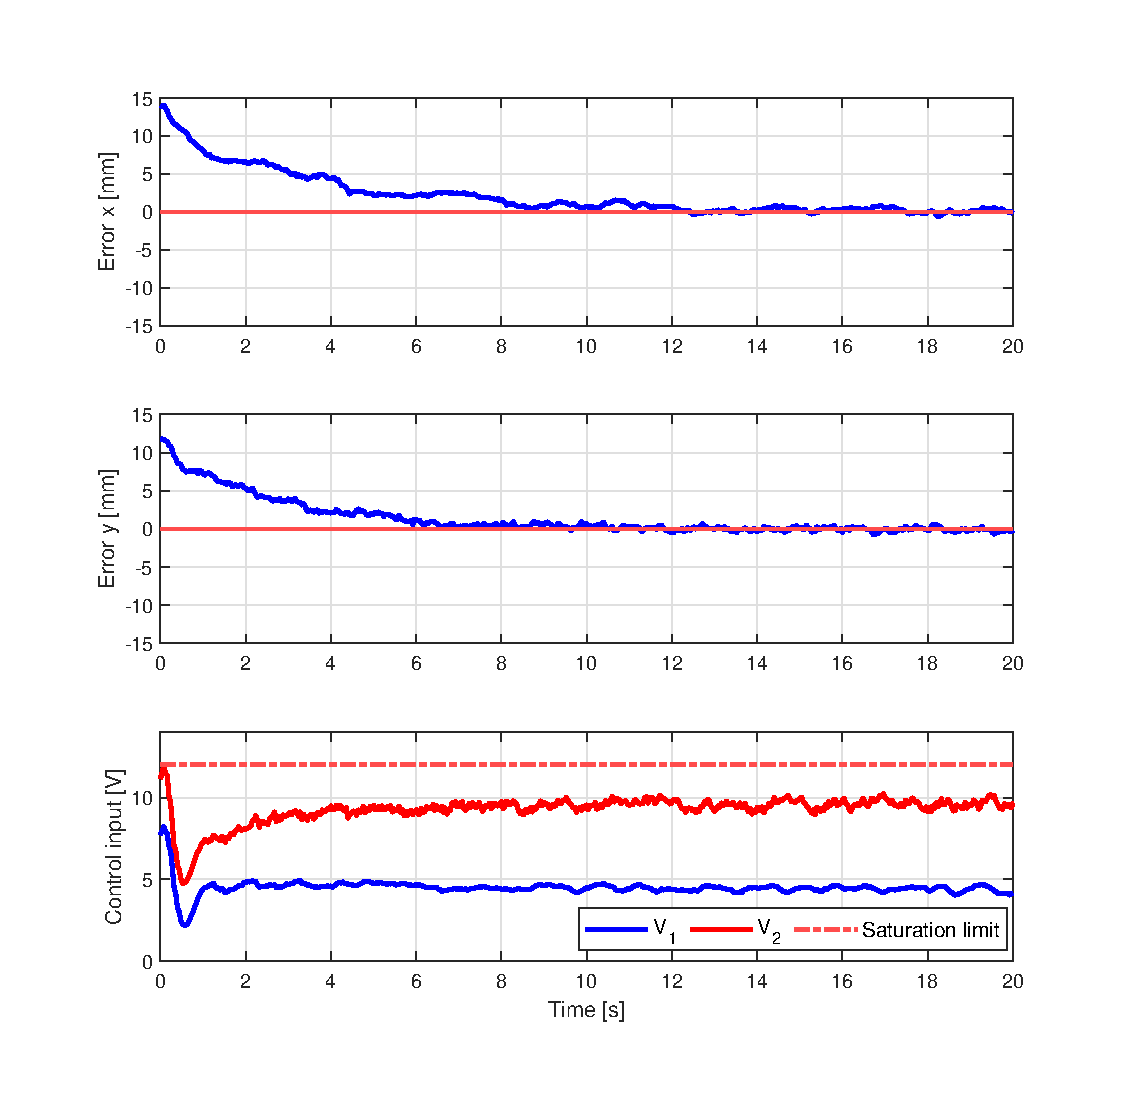
\includegraphics[width = 0.78\textwidth]{Figures/Chapter5/errorsignalright.eps}
    \caption{\textbf{Top:} Error response of the x-coordinate. \textbf{Centre:} Error response of the y-coordinate. \textbf{Bottom:} Control input signal to the air-pumps.}
    \label{fig5:stepleft}
\end{figure}

\begin{figure}[H] 
    \begin{minipage}[b]{0.49\linewidth}
     \centering
    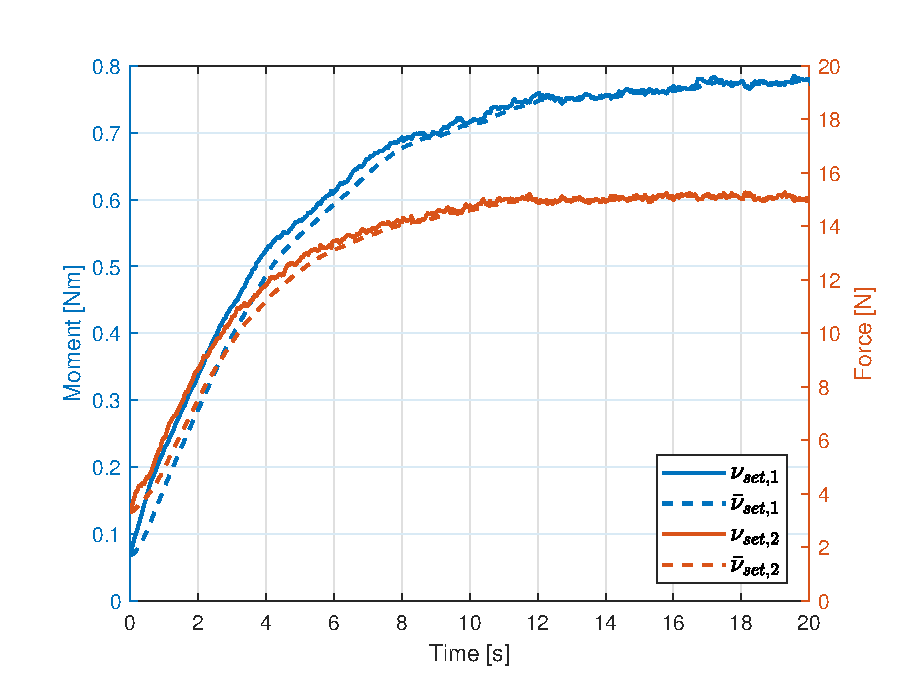
\includegraphics[width=\linewidth]{Figures/Chapter5/nuright.eps} 
    \caption{Input moment and force as determined by Jacobian controller. Solid line is unfiltered input, dotted line low-pass filtered. } 
    \label{fig3:dim} 
       \end{minipage} 
    \begin{minipage}[b]{0.49\linewidth}
     \centering
    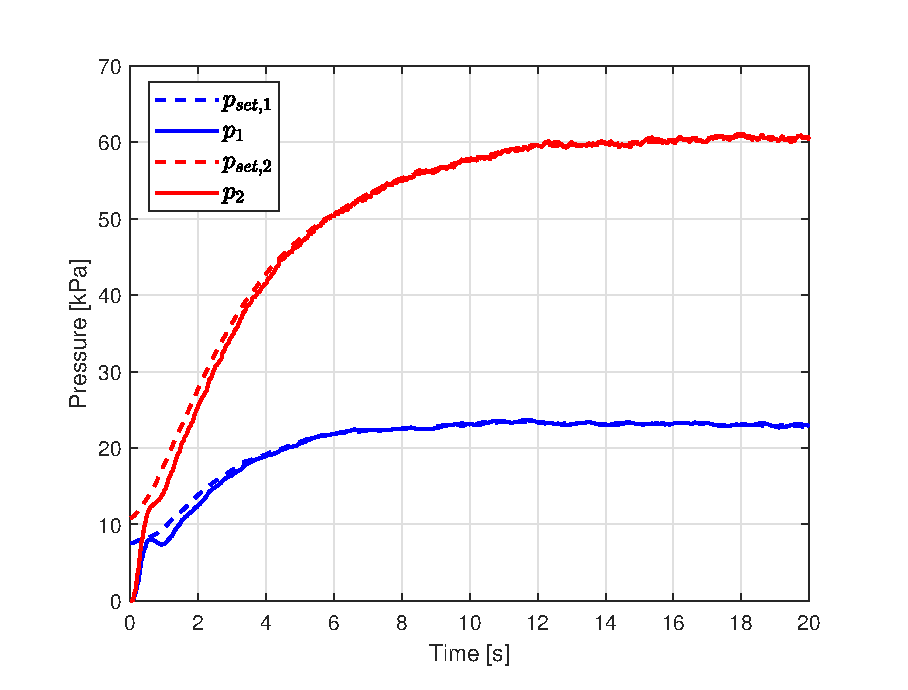
\includegraphics[width=\linewidth]{Figures/Chapter5/pressureright.eps} 
    \caption{Pressure response, dotted lines indicate reference pressure, solid lines are measured pressures.} 
    \label{fig3:FemModel} 
    \end{minipage} 
\end{figure}






\begin{table}[H]
    \centering
    \caption{RMS error after 15 seconds}
    \begin{tabular}{|c|c|c|} \hline
     Set point $[x,y]^\top$    & $e_{RMS,x}$ $mm^2$  &  $e_{RMS,y}$ $mm^2$  \\ \hline
    Left $r_{set}= [-0.014,0.082]^\top$     & 2.6034e-04  & 2.2644e-04 \\ \hline
    Right $r_{set}= [0.014,0.082]^\top$  & 3.4380e-04 &  2.8172e-04\\ \hline
    \end{tabular}

    \label{tab:my_label}
\end{table}






\section{Reference tracking in experiments}
















% Sample frequency arduino = 25 millisecond is 40 Hz Sample frequency Raspberry pixymon onn= 58 millisecond = 18.5HzSample freq Raspberyy pixymon off = 40 millisecondsPixymon off max sample freq = 40Hz, 25 millisecondpixymon on max sample freq = 20 Hz, 50 millisecond